\chapter*{Appendix}
\section{Unused plots}
\label{App:Plots}
\begin{figure}[H]
    \centering
    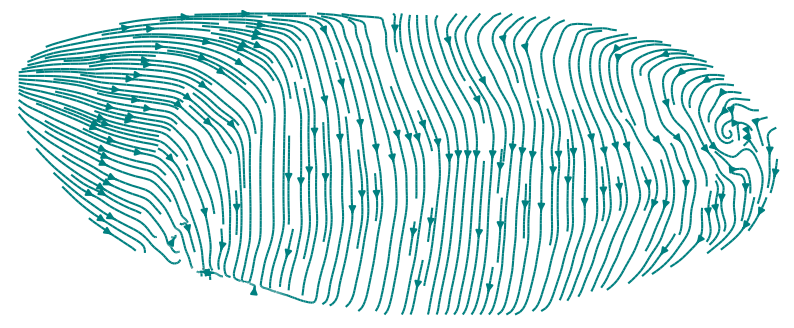
\includegraphics[width=1\linewidth]{chapters/Appendix/streamplot1.png}
\end{figure}


\begin{figure}[H]
    \centering
    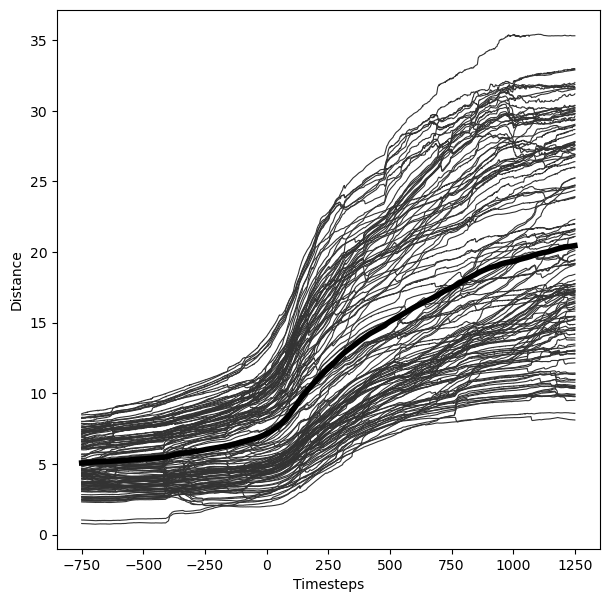
\includegraphics[width=1\linewidth]{chapters/Appendix/germbandMovementQuant.png}
    \caption{Horizontal-position of a line of germ-band cells, mirroring the analysis in  \url{https://www.ncbi.nlm.nih.gov/pmc/articles/PMC2801059/}}
    \label{fig:enter-label}
\end{figure}
\begin{figure}[H]
    \centering
    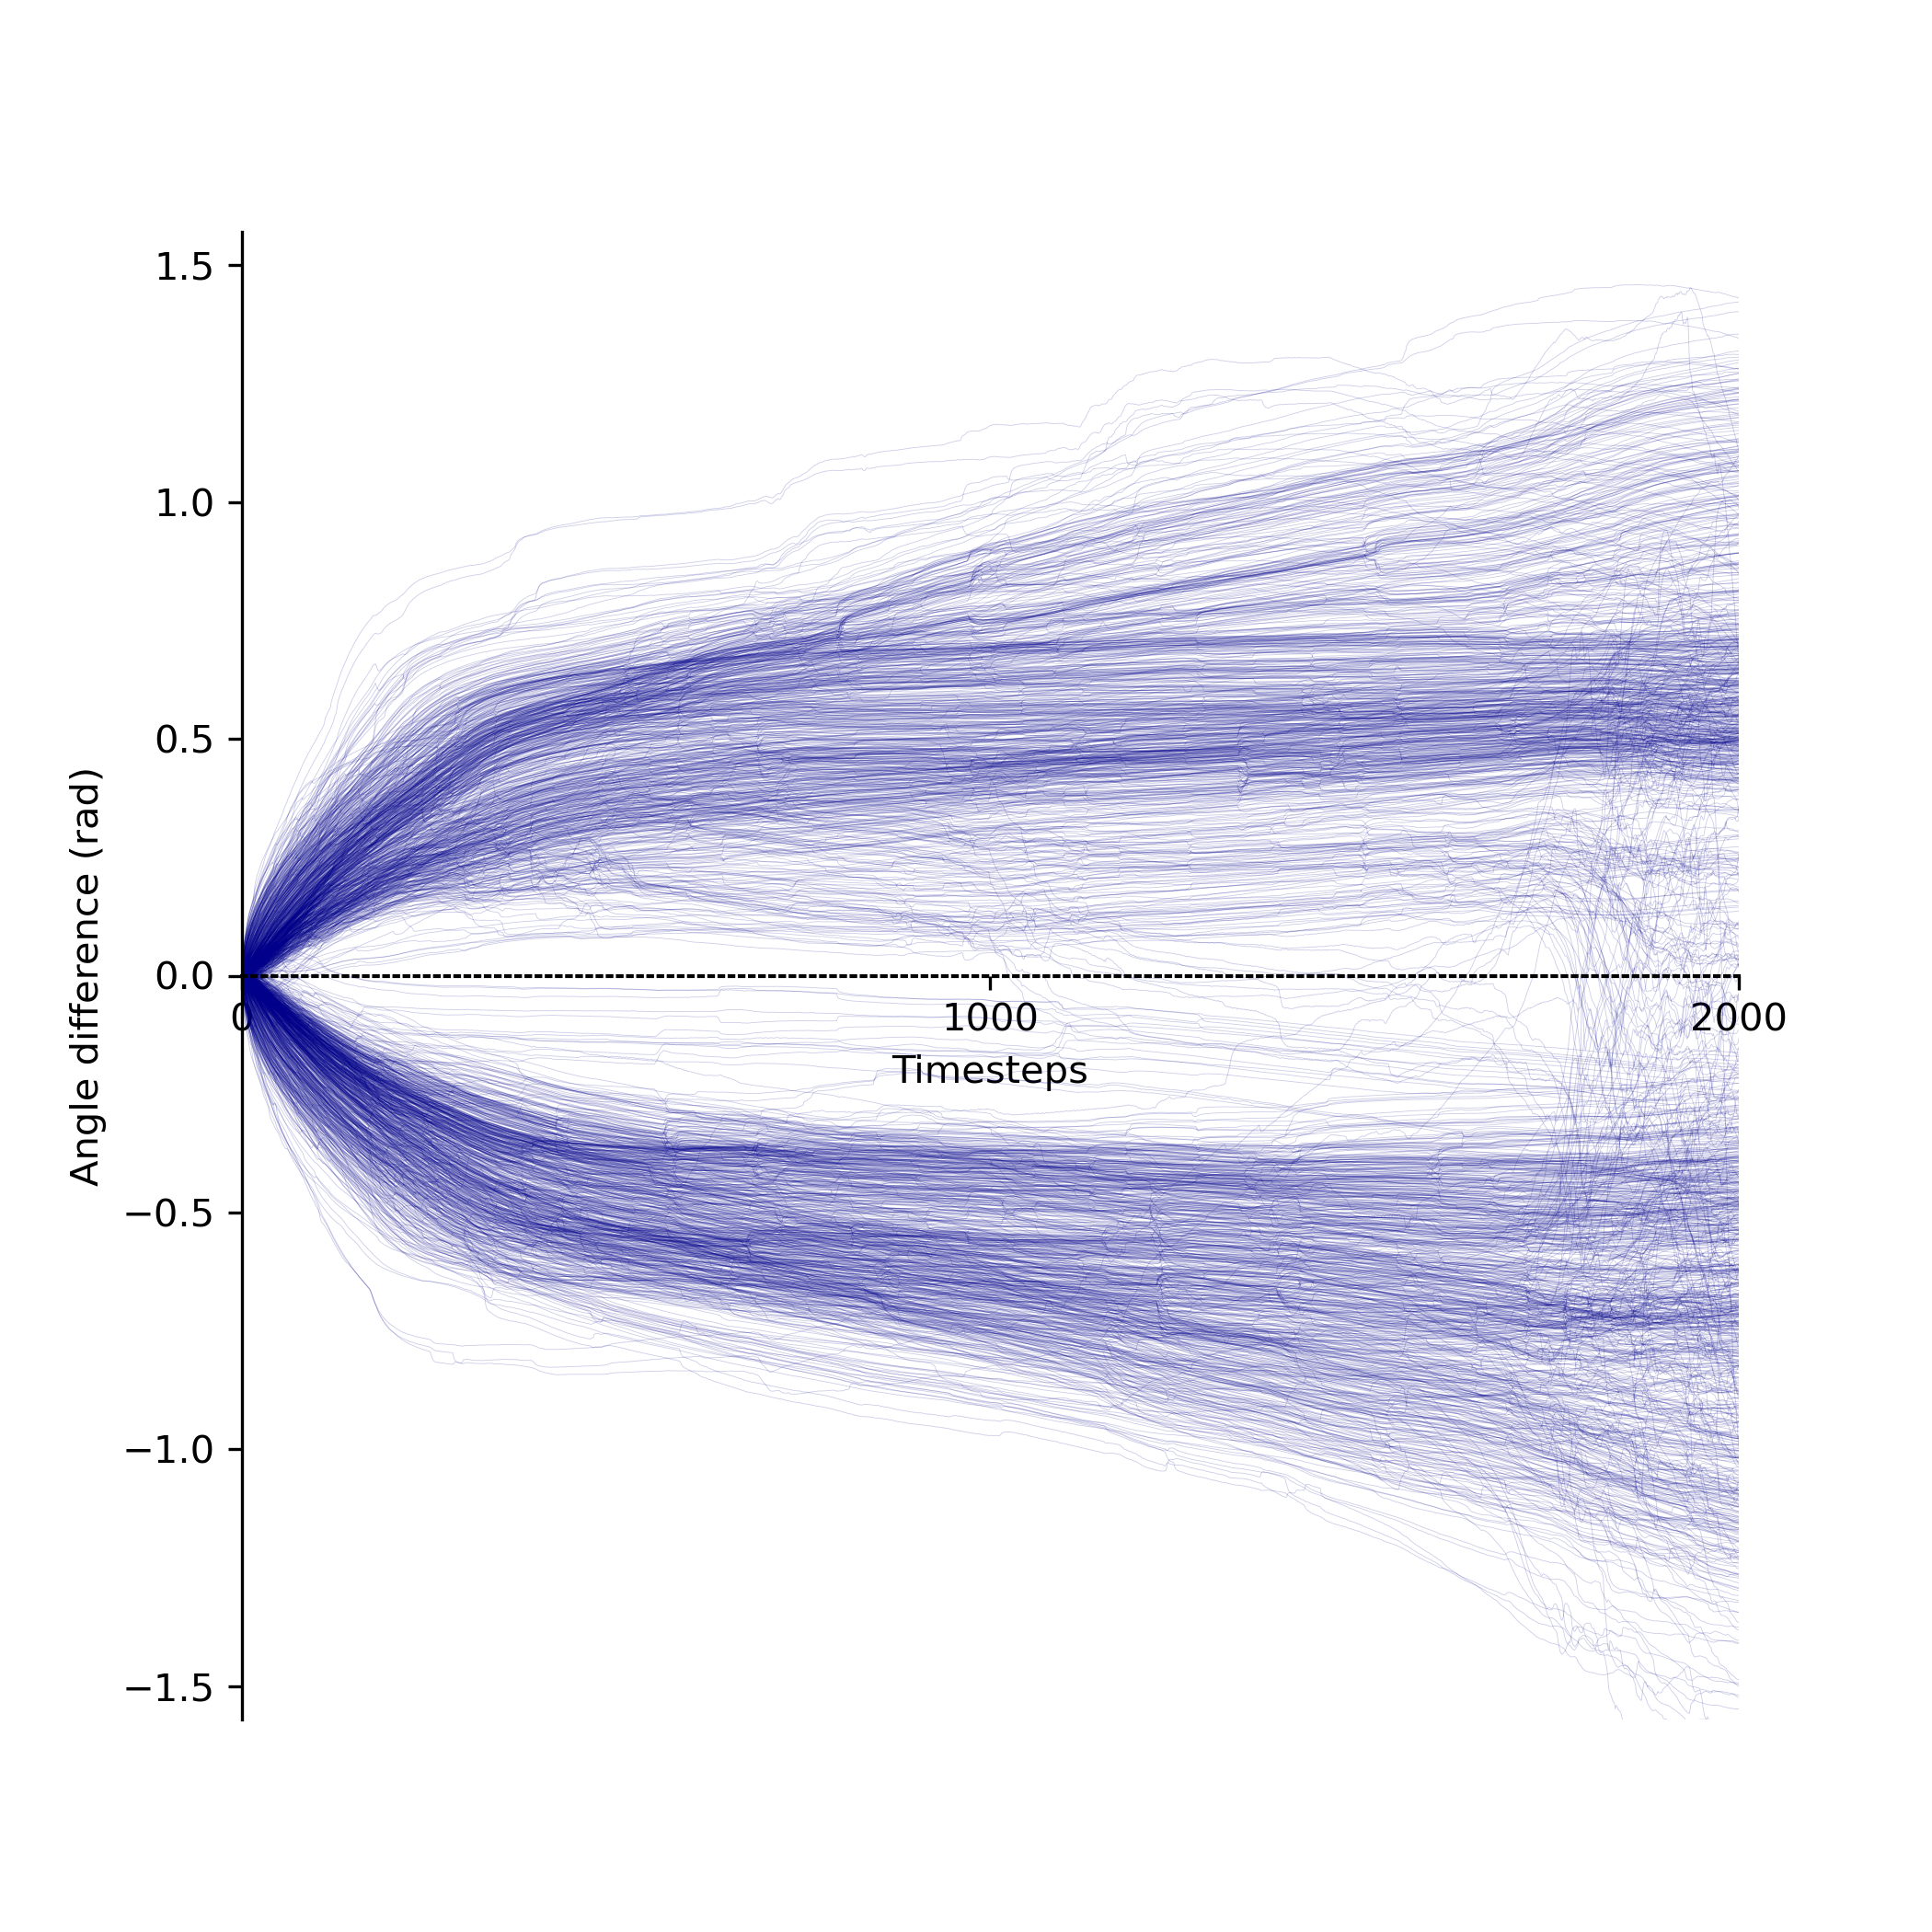
\includegraphics[width=1\linewidth]{chapters/Appendix/the_ring.png}
    \caption{Angle in cylindrical coordinates of germ-band. Mirroring \url{https://www.ncbi.nlm.nih.gov/pmc/articles/PMC2801059/}}
    \label{fig:enter-label}
\end{figure}
\section{Code details}
\label{App:Code}
\section{Additional Videos}
\label{App:videos}
\section{Sergei-analyses (tie into PCP)}
\label{App:Sergei}
\section{Green-Lagrange strain inference}
\label{App:Strain-Calculation}
Firstly transform into cylindrical coordinates.... \\
"A strain rate is the ratio of the change in length to the original length, divided by the time interval, with units of proportion (pp) per minute. The lines show the mean strain rates for all five embryos, and the ribbon width represents the average standard error within a data set. The timing of developmental landmarks is shown for the five embryos recorded"\cite{butler2009cell}
\section{Why our rosettes behave differntly }
\label{App:why-rosettes}
In our model, where the equilibrium distance is the same for every direction no matter the pressure exerted, getting a bimodality is predictable.
Every time a new pair 'touch' on the up-down axis, they release space for a pair above or below on the perpendicular axis. 


\section{We have not taking the following into account}
\subsection*{Cell shape change!}
\subsection*{Mitotic pressure in cephalic area}
\subsection*{Things that change over time}
\subsection*{Pressure-buckling of dorsal folds}
\subsection*{Pressure from yolk}
\section{Detailed morphogens}
\label{App:morphogens}
\begin{table}[H]
\begin{tabular}{lll}
 \begin{tabular}[c]{@{}l@{}}Genetically patterned \\ transcription factor proteins\end{tabular} & Location at gastrulation & Vital for development of \\ \hline
 Twist \& Snail                                                                                 & Ventral                  & Mesoderm                 \\
Huckebein \& Tailless                                                                          & Posterior                & Endoderm (Midgut)   \\

 Runt \& Even skipped & Germ Band & All of the above\\
Buttonhead \& Even skipped  & Cephalic furrow & Chephalic furrow\\

\end{tabular}
    \caption{The most important morphogens and their simplified reason of significance}
    \label{tab:morphogens}
\end{table}


\begin{lstlisting}
# The germ band requires striping to be active [citation]
GB = GE.or_gene(GE.gene("eve"), GE.gene("run"))

# A cutoff was needed because of spotty coverage
# As can be seen on all, the germ-band does not extend far up
# we expect some inhibiting gene to be doing this IRL
GB[GE.base[:,2] > 50] = 0

# remove in the head domain
GB = GE.not_gene(GB, GE.gene("fkh"))

# Add to embryo
GE.add_expression(GB, 0.2, True, 1)  # Germ Band


# Dorsal fold 1
GE.add_expression(GE.get_second_run_stripe(), 0.4, True, 5)  # Second Run Stripe

# Dorsal fold 2
GE.add_expression(GE.get_fifth_run_stripe(), 0.4, True, 5)  # Second Run Stripe

# GE.add_expression(GE.not_gene(GE.or_gene(GE.gene("eve"), GE.gene("run")), GE.gene("Doc2")), 0.2, True, 1)  # Germ Band

# add cephalic furrow
GE.add_expression(GE.gene("Dfd"), 0.6, True, 5)  # Cephalic Furrow


# combine twist and snail (twist overlaps snail completely)
twist_and_snail = GE.and_gene(GE.gene("twi"), GE.gene("sna"))

GE.add_expression(twist_and_snail, 0.2, True, 2)  # Ventral Furrow

# add posterior midgut
GE.add_expression(GE.gene("hkb"), 0.25, True, 4)  # PMG

# hkb is expressed both for the Anterior and Posterior invagination
# croc and oc are in the cephalic domain, so I use these to set 
# everything in head region back to cell type 0
GE.add_expression(GE.or_gene(GE.gene("croc"), GE.gene("oc")), 0.4, True, 0)  # Invert

# Define the PCP from the gradient of the runt gene and save
GE.save("no_q_from_runt", q_from_runt=True)
\end{lstlisting}

\subsubsection{Cell types extracted from data}
When we say that the cell types were extracted from data, this comes with a couple asterisks:\\
Any expression in the cephalic region was removed by hand.\\
\textbf{Cephalic furrow}
In the data-set there were no [Cephalic furrow gene], but using the website [website] we could see that it spatially coincided with [other gene] which was in the data-set and was therefore used as a proxy. 
\textbf{Germ-band}
The germ-band was cut off by hand as the [gene1] and [gene2] expressions were very spotty at the top and the germ-band would not extend correctly.\footnote{I am guessing a suppressing gene that we did not take into account is also at play} 

\textbf{Ventral furrow}
Even though all the cells expressing \textit{twist} \& \textit{snail} on the belly lower their apical surface area, they do not constrict indiscriminately. Instead they start out by constricting in the \textit{inner} 8x60 cells. [citation needed] It is believed to be a more stable way of wedging [citation needed] but is still strange and not fully understood. [citation needed]. This meant that a specific rule for the wedging in the ventral region was needed. The inner 8 cells has a wedging constant $\alpha = 0.5$ while the rest has $\alpha = 0.2$.

\section*{Rosette analysis}
Convergent Extension is seen as a vital part of the development of many different YYY. Therefore multiple different methods of analysis and YYY have been developed.
One of the main quantifiers consist of looking at a cluster of neighboring cells that undergo convergent extension. These clusters are called Rosettes. Trough laser-ablation is has been shown that the Rosettes (as shown in the diagram on Figure \ref{fig:ConvergentExtensionDiagram}) can consist of up two twelve internally connected cells [citation needed].
For drosophila gastrulation in particular, the direction between each newly acquired neighbor is \todo{finish thought}



% \begin{figure}[H]
%     \centering
%     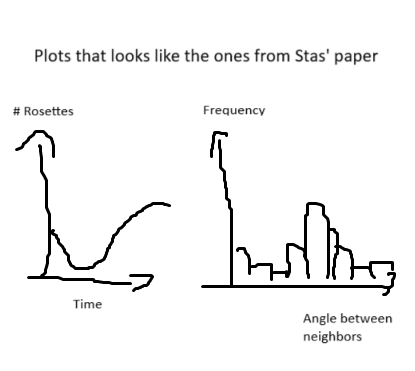
\includegraphics[width=0.8\linewidth]{chapters/Results/figures/rosettes_placeholder.png}
%     \caption{Caption}
%     \label{fig:enter-label}
% \end{figure}


\begin{figure}[H]
    \centering
    \makebox[\textwidth][c]{
    \begin{subfigure}[b]{0.55\textwidth}
    \centering
        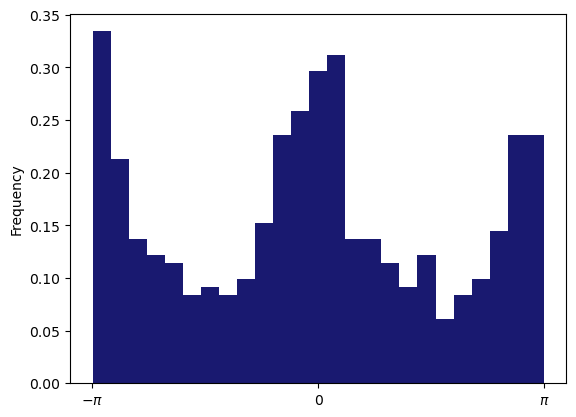
\includegraphics[width=\linewidth]{chapters/Results/figures/rosettes_angle_dist.png}

    \end{subfigure}
    \begin{subfigure}[b]{0.5\textwidth}
    \centering
    
    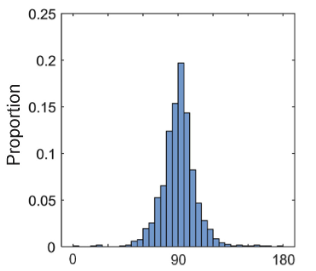
\includegraphics[width=\linewidth]{chapters/Results/figures/rosettes_angle_dist_data.png}
    \end{subfigure}
    }
    \caption{The angular distribution of the newly acquired neighbors in rosettes as found in (\textbf{left}) simulation (in radians) and (\textbf{right}) data (in degrees).}
    \label{fig:roestte-angle-dist}
    
\end{figure}
In Figure \ref{fig:roestte-angle-dist}, the distribution of angles of all found rosette-events can be seen. Strangely, the distribution is clearly bimodal in horizontal and vertical, where the ground truth has a single peak at the vertical axis. 

We believe the lack of malleability in the contours of the cells might be to blame.


% When speaking with Daniel, a researcher at the [Stas'] laboratory who did the original analysis, he said that this makes sense, as looking at neighboring nuclei is fundamentally different from edges. \todo{rephrase to make less bad}. 

% I won't bore you the details, so a quick run-down of our thoughts and discussions can be found in Section \ref{App:why-rosettes} in the Appendix.\\

% ... \\
% Speaking of Daniel:
\note{
Not showing something good :( Keep for completeness or move to appendix?}

% \subsection{Daniel-data?}
% Nothing here yet...
% \begin{figure}[H]
%     \centering
%     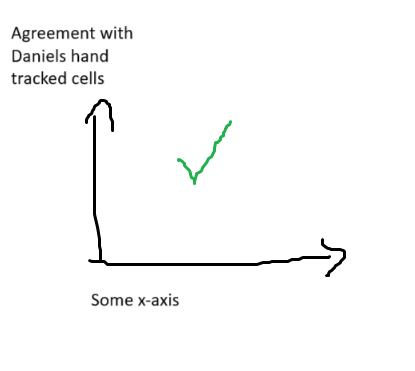
\includegraphics[width=0.7\linewidth]{chapters/Results/figures/daniel_placeholder.png}
%     \caption{Some caption}
%     \label{fig:enter-label}
% \end{figure}

\section*{Other efforts we have tried in vain}
\section*{For eftertiden}
\subsection{Ventral Furrow}
I would love to quantify the accuracy of our simulated ventral furrow.\\
I am guessing we can do a cell-center fit of Figure \ref{fig:VFComparison}.\\
Is this out of scope? Yes. Would it be cool? Also yes.

\subsection{Cell surface area}
I am sure I could get the data and would love to quantify the agreement.

\subsection{Interaction matrix}
Wish I had time

\subsection{Without gene-defined pcp}
Wish I had time

